\subsection{Introduction}

Conclusions often echo introductions. This chapter was completed at the very end of the writing of the book. It outlines principles and ideas that are probably more relevant than the sum of technical details covered subsequently. When stuck with disappointing results, we advise the reader to take a step away from the algorithm and come back to this section to get a broader perspective of some of the issues in predictive modelling.

\subsubsection{Context}

The blossoming of machine learning in factor investing has it source at the confluence of three favorable developments: data availability, computational capacity, and economic groundings.

First, the \textbf{data}. Nowadays, classical providers, such as Bloomberg and Reuters have seen their playing field invaded by niche players and aggregation platforms. In addition, high-frequency data and derivative quotes have become mainstream. Hence, firm-specific attributes are easy and often cheap to compile. This means that the size of $\mathbf{X}$ in Equation \ref{superv} below is was already sufficiently large in 2020 (first edition of the book) to be plugged into ML algorithms. The order of magnitude (in 2027, it has not changed much from 2019 in fact) that can be reached is the following:

\begin{itemize}
\item a few hundred monthly observations (a handful decades)
\item over several thousand stocks (US listed at least)
\item covering a several hundred attributes (sometimes a few thousand, but with possible colinearity).
\end{itemize}

This implies datasets of dozens of millions of points or more. While it is a reasonably high figure, we highlight that the chronological depth is probably the weak point and will remain so for decades to come because accounting figures are only released on a quarterly basis. This can somewhat be alleviated when generating synthetic data, though the efficiency of such strategy remains to be demonstrated. Needless to say that this drawback does not hold for high-frequency strategies that rely on intraday data (out of the scope of the present monograph).

Second, \textbf{computational power}, both through hardware and software. Storage and processing speed are not technical hurdles anymore and models can even be run on the cloud thanks to services hosted by major actors (Amazon, Microsoft, IBM and Google) and by smaller players (Rackspace, Techila). On the software side, open source has become the norm, funded by corporations (TensorFlow \& Keras by Google, Pytorch by META/Facebook, h2o, etc.), universities (Scikit-Learn by INRIA, NLPCore by Stanford, NLTK by UPenn) and small groups of researchers (caret, xgboost, catboost, lightGBM, tidymodels to list but a pair of frameworks). Consequently, ML is no longer the private turf of a handful of expert computer scientists, but is on the contrary \textbf{accessible} to anyone willing to learn and code. Moreover, with the advent of Large Languages Models, coding has never been easier.

Finally, \textbf{economic framing}. Machine learning applications in finance were initially introduced by computer scientists and information system experts (e.g., \citep{braun1987predicting}, \citep{white1988economic}) and exploited shortly after by academics in financial economics (\citep{bansal1993no}), and hedge funds (see, e.g., \citep{zuckerman2019man}). Nonlinear relationships then became more mainstream in asset pricing (\citep{freeman1992nonlinear}, \citep{bansal1993new}). These contributions started to pave the way for the more brute-force approaches that have blossomed since the 2010 decade and which are mentioned throughout the book.

In the synthetic proposal of \citep{arnott2019backtesting}, the first piece of advice is to rely on a model that makes sense economically. We agree with this stance, and the only assumption that we make in this book is that future returns depend on firm characteristics. The relationship between these features and performance is largely unknown and probably time-varying. This is why ML can be useful: to detect some hidden patterns beyond the documented asset pricing anomalies. Moreover, dynamic training allows to adapt to changing market conditions.

\subsubsection{Portfolio construction: the workflow}

Building successful portfolio strategies requires many steps. This book covers many of them but focuses predominantly on the prediction part. Indeed, allocating to assets most of the time requires to make bets and thus to presage and foresee which ones will do well and which ones will not. In this book, we mostly resort to supervised learning to forecast returns in the cross-section. The baseline equation in supervised learning,

\begin{equation}
\label{superv}
\mathbf{y}=f(\mathbf{X})+\mathbf{\epsilon},
\end{equation}

is translated in financial terms as

\begin{equation}
\label{superv_return}
\mathbf{r}_{t+1,n}=f(\mathbf{x}_{t,n})+\mathbf{\epsilon}_{t+1,n},
\end{equation}

where $f(\mathbf{x}_{t,n})$ can be viewed as the \textbf{expected return} for time $t+1$ computed at time $t$, that is, $\mathbb{E}_t[r_{t+1,n}]$. Note that the model is \textbf{common to all assets} ($f$ is not indexed by  $n$), thus it shares similarity with panel approaches.

Building accurate predictions requires to pay attention to \textbf{all} terms in the above equation. Chronologically, the first step is to gather data and to process it (see Chapter 4). To the best of our knowledge, the only consensus is that, on the $\textbf{x}$ side, the features should include classical predictors reported in the literature: market capitalization, accounting ratios, risk measures, momentum proxies (see Chapter 3). For the dependent variable, many researchers and practitioners work with monthly returns, but other maturities may perform better out-of-sample.

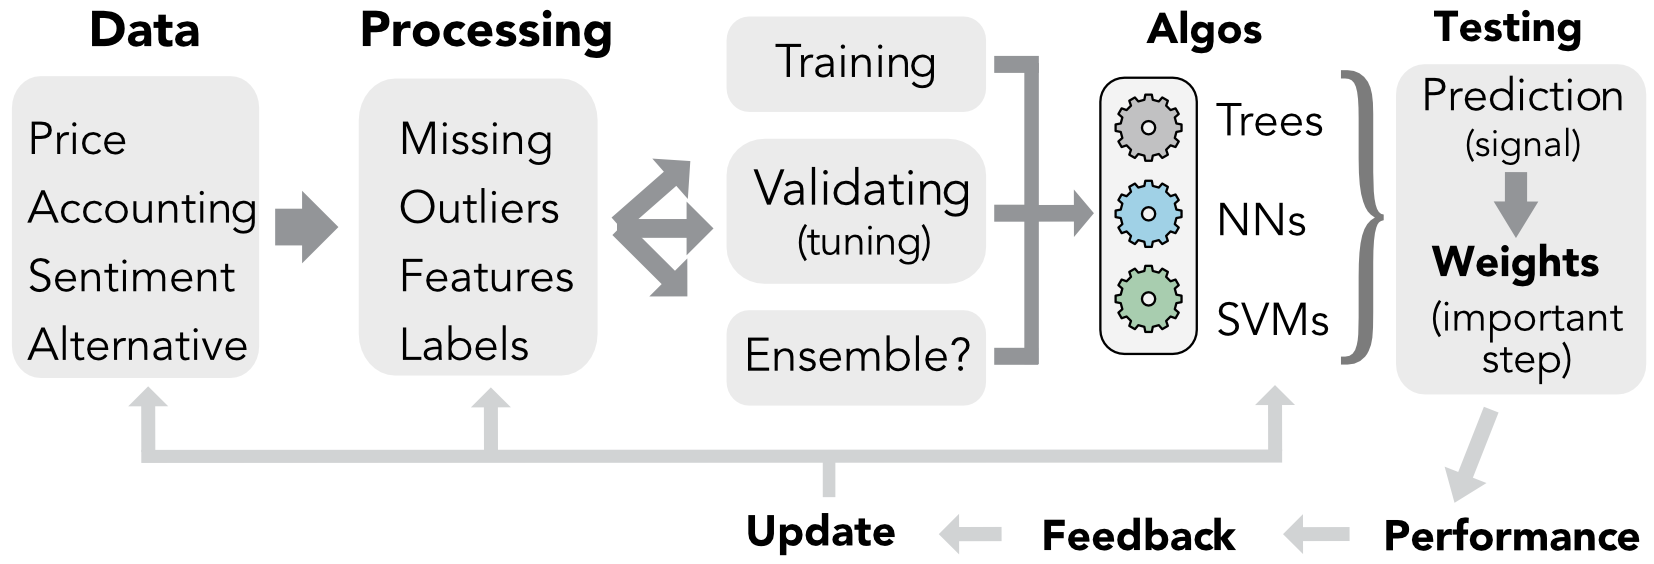
\includegraphics[width=0.7\linewidth]{files/scheme2_big-1e5ed17e728c0d450ddca5c5b6fa11ce.png}


Simplified workflow in ML-based portfolio construction.

\subsubsection{Machine Learning is no magic wand}

By definition, the curse of predictions is that they rely on \textbf{past} data to infer patterns about \textbf{subsequent} fluctuations. The more or less explicit hope of any forecaster is that the past will turn out to be a good approximation of the future. Needless to say, this is a pious wish; in general, predictions fare badly. Surprisingly, this does not depend much on the sophistication of the econometric tool. In fact, heuristic guesses are often hard to beat.

To illustrate this sad truth, the baseline algorithms that we detail in Chapters 5 to 7 yield at best mediocre results. This is done \textbf{on purpose}. This forces the reader to understand that blindly feeding data and parameters to a coded function will seldom suffice to reach satisfactory out-of-sample accuracy.

In machine learning, models are estimated on one portion of data (\textbf{training set}) and then tested on another portion of the data (\textbf{testing set}) to assess their quality. We split our sample accordingly.

Below, we sum up some key points that we have learned through our exploratory journey in financial ML.

\begin{itemize}
\item The first point is that \textbf{causality} is key. If one is able to identify $X \rightarrow y$, where $y$ are expected returns, then the problem is solved. Unfortunately, causality is incredibly hard to uncover.
\item Thus, researchers have most of the time to make do with simple \textbf{correlation} patterns, which are far less informative and robust.
\item Relatedly, financial datasets are extremely noisy. It is a daunting task to \textbf{extract signals} out of them. \textbf{No-arbitrage} reasonings imply that if a simple pattern yielded durable profits, it would mechanically and rapidly vanish.
\item The no-free lunch theorem of \citep{wolpert1992connection} imposes that the analyst formulates views on the model. This is why economic or \textbf{econometric framing} is key. The assumptions and choices that are made regarding both the dependent variables and the explanatory features are decisive. As a corollary, data is key. The inputs given to the models are probably much more important than the choice of the model itself.
\item To maximize out-of-sample efficiency, the right question is probably to paraphrase Jeff Bezos: what's not going to change? \textbf{Persistent} series are more likely to unveil enduring patterns.
\item Everybody makes mistakes. Errors in loops or variable indexing are part of the journey. What matters is to \textbf{learn} from those lapses.
\end{itemize}

To conclude, we remind the reader of this obvious truth: nothing will ever replace \textbf{practice}. Gathering and cleaning data, coding backtests, tuning ML models, testing weighting schemes, debugging, starting all over again: these are all absolutely indispensable steps and tasks that must be repeated indefinitely. There is no sustitute to experience.